% !TEX program = lualatex
% ============================================================================
% Conference poster — Part III/MASt project conference (17 June 2026)
% "Amplifying graviton-photon conversion with spacetime torsion"
% William Royce, Cavendish Astrophysics.
%
% Build: LuaLaTeX REQUIRED (Gemini theme uses fontspec). The `% !TEX program`
% line above tells editors to use lualatex. From the CLI use `make` or
%   latexmk -lualatex poster.tex
% The theme/ dir is added to \input@path below so \usetheme finds the local
% theme files without needing TEXINPUTS set.
% ============================================================================
\documentclass[final]{beamer}

% Make the local theme/ directory discoverable by \usetheme / \usecolortheme
% (so a direct `lualatex poster.tex` works without TEXINPUTS=./theme).
\makeatletter
\providecommand\input@path{}
\g@addto@macro\input@path{{theme/}}
\makeatother

% ---- Poster size: A0 portrait ----------------------------------------------
\usepackage[size=a0,orientation=portrait,scale=1.15]{beamerposter}
\usetheme{gemini}
\usecolortheme{cam}

% ---- Math (no stix: amssymb \varkappa, mathrsfs \mathscr) -------------------
\usepackage{amsmath}
\usepackage{amssymb}
\usepackage{mathtools}
\usepackage{mathrsfs}
\usepackage{tensor}
\usepackage{accents}

% ---- Macro helpers required by poster-macros.tex ---------------------------
\usepackage{etoolbox}
\usepackage{xspace}
\usepackage{xstring}

% ---- Graphics / QR ---------------------------------------------------------
\usepackage{graphicx}
\usepackage{tikz}
\usetikzlibrary{arrows.meta,positioning,decorations.pathmorphing,calc}
\usepackage{qrcode}
\usepackage{anyfontsize}   % arbitrary title sizes
\graphicspath{{figures/}{theme/}}

% ---- Notation (extracted from ../macros.tex) -------------------------------
% ============================================================================
% poster-macros.tex
% Notation macros EXTRACTED from ../macros.tex for the poster build.
% Only the \newcommand notation is carried over -- the report's stix/RevTeX
% font stack is intentionally NOT loaded here (it clashes with the Gemini
% LuaLaTeX + Lato font setup). \varkappa comes from amssymb; \mathscr from
% mathrsfs. Assumes the poster preamble has loaded: amsmath, amssymb,
% mathtools, mathrsfs, tensor, accents, etoolbox, xspace, xstring.
% ============================================================================

% --- Abbreviations -----------------------------------------------------------
\newcommand*{\ie}{i.e.,\@\xspace}
\newcommand*{\eg}{e.g.,\@\xspace}

% --- Common math operators ---------------------------------------------------
\newcommand*{\qand}{\quad\text{and}\quad}
\newcommand*{\D}{D_\mathrm{KL}}
\newcommand*{\Dp}{D_\mathrm{KL,+}}
\newcommand*{\Dm}{D_\mathrm{KL,-}}

% --- Software names (italic, per Barker corpus) -------------------------------
\newrobustcmd{\TIDAL}{\textit{TIDAL}\xspace}
\newrobustcmd{\PSALTer}{\textit{PSALTer}\xspace}
\newrobustcmd{\etal}{\textit{et al.}\xspace}
\newrobustcmd{\xAct}{\textit{xAct}\xspace}
\newrobustcmd{\Mathematica}{\textit{Mathematica}\xspace}
\newrobustcmd{\Python}{\textit{Python}\xspace}

% --- Gravitational coupling --------------------------------------------------
% kappa -> varkappa (amssymb); P = sin^2(kappa B_0 D / 2)
\renewcommand{\kappa}{\varkappa}
\renewcommand{\O}{\mathcal{O}}

% --- PGT coupling constants --------------------------------------------------
\newrobustcmd{\Alp}[1]{\alpha_{#1}}
\newrobustcmd{\Bet}[1]{\beta_{#1}}
\newrobustcmd{\Gam}[1]{\gamma_{#1}}
\newrobustcmd{\Del}[1]{\delta_{#1}}

% --- Differential ------------------------------------------------------------
\newcommand{\diff}{\mathrm{d}}

% --- Covariant derivatives ---------------------------------------------------
\newrobustcmd{\rD}[1]{\tensor{\mathring{\nabla}}{#1}}   % Riemannian nabla
\newrobustcmd{\rcD}[1]{\tensor{\nabla}{#1}}             % Riemann-Cartan nabla

% --- PGT fields: torsion, curvature ------------------------------------------
\newrobustcmd{\MAGA}[1]{\tensor{\Gamma}{#1}}                    % RC connection
\newrobustcmd{\MAGT}[1]{\tensor{\mathcal{T}}{#1}}              % torsion (cal T)
\newrobustcmd{\MAGTTilde}[1]{\tensor{\tilde{\mathcal{T}}}{#1}} % traceless torsion
\newrobustcmd{\MAGF}[1]{\tensor{\mathcal{R}}{#1}}             % curvature (cal R)
\newrobustcmd{\MAGFt}[1]{\tensor{\tilde{\mathcal{R}}}{#1}}    % RC curvature (tilde)

% --- Electromagnetic fields --------------------------------------------------
\newrobustcmd{\FieldA}[1]{\tensor{A}{#1}}             % EM 4-potential
\newrobustcmd{\FieldF}[1]{\tensor{\mathcal{F}}{#1}}   % EM field strength (cal F)
\newrobustcmd{\FieldH}[1]{\tensor{h}{#1}}             % metric perturbation

% --- Gertsenshtein effect ----------------------------------------------------
\newcommand{\Bzero}{B_0}              % background magnetic field
\newcommand{\Pconv}{P_{g\gamma}}      % photon-graviton conversion probability
\newcommand{\Pmax}{P_\mathrm{max}}    % maximum conversion probability

% --- Lagrangian / Hamiltonian densities --------------------------------------
\newcommand{\lag}{\mathscr{L}}
\newcommand{\ham}{\mathscr{H}}
\newcommand{\act}{\mathscr{S}}


% ---- Block body padding: indent text inside the filled (contained) boxes ----
% Gemini's standard block body has no side padding; add it so the light-blue
% boxes read as properly contained (the alerted/example blocks already pad).
\setbeamertemplate{block begin}{
  \begin{beamercolorbox}[colsep*=0ex,dp=2ex,center]{block title}
    \vskip0pt
    \usebeamerfont{block title}\insertblocktitle
    \vskip-1.25ex
    \begin{beamercolorbox}[colsep=0.025ex]{block separator}\end{beamercolorbox}
  \end{beamercolorbox}
  {\parskip0pt\par}
  \usebeamerfont{block body}
  \vskip-0.5ex
  \begin{beamercolorbox}[colsep*=0ex]{block body}
  \justifying
  \begin{adjustwidth}{1.5ex}{1.5ex}
  \setlength{\parskip}{1ex}
  \vskip0.5ex
}
\setbeamertemplate{block end}{
  \vskip0.5ex
  \end{adjustwidth}
  \end{beamercolorbox}
  \vskip0pt
  \vspace*{2ex}
}

% ---- Header typography: large full-width title ------------------------------
\setbeamerfont{headline title}{size=\fontsize{104}{116}\selectfont,series=\bfseries}
\setbeamerfont{headline author}{size=\LARGE,series=\bfseries}
\setbeamerfont{headline institute}{size=\large}

% ---- Custom headline: standard-blue top bar -> light-blue title field ->
%      BOLD warm-blue separation rule (mirrors the Cambridge talk frametitle). ----
\setbeamertemplate{headline}{%
  % (1) standard-blue bar across the very top
  \begin{beamercolorbox}[wd=\paperwidth,ht=1.6ex,sep=0pt]{headline topbar}\end{beamercolorbox}%
  \nointerlineskip
  % (2) light-blue header field with title / author / institute
  \begin{beamercolorbox}[wd=\paperwidth,sep=0pt]{headline}%
    \vskip2.0ex
    \centering
    {\usebeamerfont{headline title}\usebeamercolor[fg]{headline title}\inserttitle\par}
    \vskip1.6ex
    {\usebeamerfont{headline author}\usebeamercolor[fg]{headline author}\insertauthor\par}
    \vskip0.7ex
    {\usebeamerfont{headline institute}\usebeamercolor[fg]{headline institute}\insertinstitute\par}
    \vskip2.0ex
  \end{beamercolorbox}%
  \nointerlineskip
  % (3) BOLD warm-blue rule separating header from body
  \begin{beamercolorbox}[wd=\paperwidth,ht=1.1ex,sep=0pt]{headline rule}\end{beamercolorbox}%
}

% ---- Layout lengths (3-column grid) ----------------------------------------
\newlength{\sepwidth}
\newlength{\colwidth}
\setlength{\sepwidth}{0.025\paperwidth}
\setlength{\colwidth}{0.300\paperwidth}
\newcommand{\separatorcolumn}{\begin{column}{\sepwidth}\end{column}}

% ---- Metadata --------------------------------------------------------------
% Title spans (almost) the full width; forced 2-line break for balance. No
% subtitle in the header.
\title{\parbox{0.92\paperwidth}{\centering
  Amplifying graviton--photon conversion\\ with spacetime torsion}}
\author{William Royce}
% Affiliation constrained to 70% width (centred) so the long lines clear the
% logo sitting in the free top-right corner of the header.
\institute{\parbox{0.60\paperwidth}{\centering
  {\normalfont\itshape Supervised by} W.~E.~V.~Barker, M.~P.~Hobson \& A.~N.~Lasenby\\[0.2ex]
  Astrophysics Group, Cavendish Laboratory, University of Cambridge}}

% Logo overlaid on the right, LOWERED to sit in the free space beside the centred
% author/affiliation block (the title now uses the full width above it).
\addtobeamertemplate{headline}{}{%
  \begin{tikzpicture}[remember picture,overlay]
    \node[anchor=north east, inner sep=0pt]
      at ([xshift=-4cm,yshift=-8.5cm]current page.north east)
      {
\includegraphics[height=4.4cm]{uc-cmyk}};
  \end{tikzpicture}%
}

% Footer band is rendered as the lowest content section (Cambridge-Blue band with
% warm-blue top rule + QR), so the Gemini bottom footline strip is left empty.

% ============================================================================
\begin{document}
\begin{frame}[t]

% ---- Row 1: full-width key finding -----------------------------------------
\begin{columns}[t]
  \separatorcolumn
  \begin{column}{\dimexpr\paperwidth-2\sepwidth\relax}
    % Key finding (cherry) — the bare-minimum takeaway: the headline sentence as the
% box title, plus ONE short sentence. (Highlights carries the next level of detail.)
\begin{alertblock}{Spacetime torsion can strongly amplify the conversion of
    gravitational waves into photons}
  \centering
  Across the operator landscape of Poincar\'e gauge theory we find both
  ghost-free amplification and suppression of the conversion, and we identify
  a $\MAGF{}\times\rcD{}\MAGT{}$ interaction as the dominant amplifying operator.
\end{alertblock}

  \end{column}
  \separatorcolumn
\end{columns}

% ---- Row 2: highlights (1 col) + graphical abstract (2 cols) ----------------
\begin{columns}[t]
  \separatorcolumn
  \begin{column}{\colwidth}
    % Highlights box: 3 one-line take-homes (Crowe device, near the top).
\begin{block}{Highlights}
  \begin{itemize}
    \item The standard graviton$\leftrightarrow$photon (\emph{Gertsenshtein})
          effect is far too weak to ever observe.
    \item \TIDAL{} lets us scan \emph{any} gravity theory for amplification,
          straight from its Lagrangian.
    \item Across theories with torsion we find significant, \textbf{ghost-free}
          amplification --- carried by a single curvature--torsion coupling
          $\MAGF{}\!\times\!\rcD{}\MAGT{}$.
  \end{itemize}
\end{block}

  \end{column}
  \separatorcolumn
  \begin{column}{\dimexpr2\colwidth+\sepwidth\relax}
    % Graphical abstract = hero visual (the 30-second pitch).
\begin{block}{The idea in one picture}
  \centering
  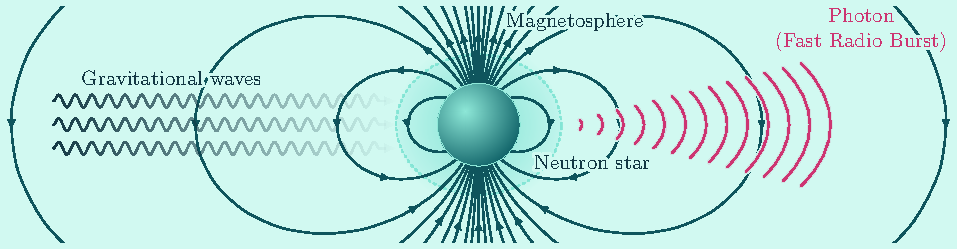
\includegraphics[width=0.95\linewidth]{magnetar_conversion.pdf}\\[0.5ex]
  {\normalsize Gravitational waves crossing the magnetic field of a neutron star
   convert into photons. In general relativity the effect is negligible; modified
   gravity with \emph{torsion} can amplify it.}
\end{block}

  \end{column}
  \separatorcolumn
\end{columns}

% ---- Row 3: the three main sections ----------------------------------------
\begin{columns}[t]
  \separatorcolumn
  \begin{column}{\colwidth}
    % Section 1 — Why it matters.
\begin{block}{1.\quad Why it matters}
  High-frequency gravitational waves --- from the early Universe and exotic
  compact sources --- have \emph{no} established detector. The
  \emph{Gertsenshtein effect}, where a gravitational wave converts into a
  photon inside a magnetic field $\Bzero$, is one of the few proposed windows.

  \vspace{1ex}
  In Einstein--Maxwell gravity the conversion probability is
  \begin{exampleblock}{}
    \centering\large
    $\Pconv = \sin^2\!\big(\tfrac{1}{2}\kappa\,\Bzero D\big)$
  \end{exampleblock}
  which is \textbf{astrophysically negligible} ($\Pconv\!\sim\!10^{-10}$ even at
  magnetar fields). \emph{Any observable signal demands new physics} --- so the
  question is \emph{which} extension of gravity could amplify it.
\end{block}

  \end{column}
  \separatorcolumn
  \begin{column}{\colwidth}
    % Section 2 — How: scan any theory (TIDAL).
\begin{block}{2.\quad How: scan any theory}
  The space of gravity theories with torsion (\emph{Poincar\'e gauge theory}) is
  vast --- far too large to work through by hand. We built \TIDAL{}, which
  automates the whole chain:
  \vspace{1ex}
  \begin{center}
    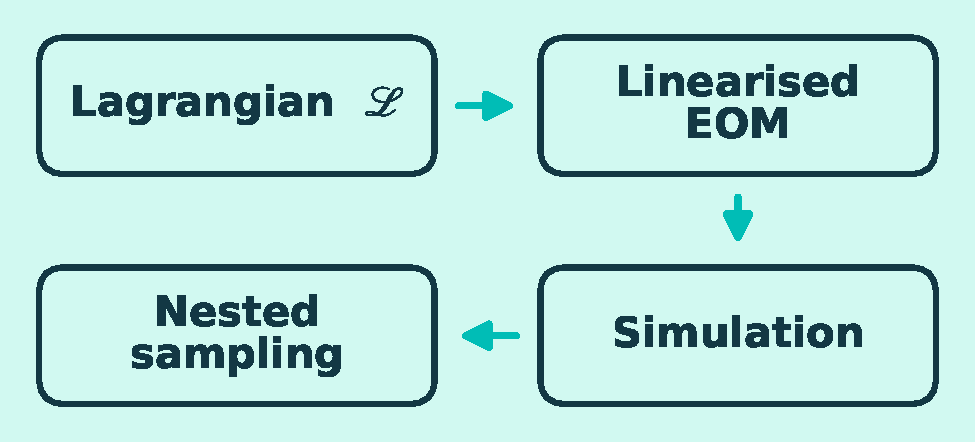
\includegraphics[width=\linewidth]{pipeline_schematic.pdf}
  \end{center}
  \vspace{0.5ex}
  Starting from a \emph{Lagrangian}, \TIDAL{} derives the linearised equations
  of motion symbolically (\xAct{}), evolves them with a fast spectral solver,
  and uses Bayesian nested sampling to map \emph{where} in coupling space the
  conversion is amplified versus suppressed, relative to the Einstein--Maxwell
  baseline.
\end{block}

  \end{column}
  \separatorcolumn
  \begin{column}{\colwidth}
    % Section 3 — What we found (double-width box: big figure left, text/eqn right).
\begin{block}{3.\quad Ghost-free amplification and suppression}
  \begin{columns}[c]
    % --- big corner figure ---
    \begin{column}{0.60\linewidth}
      \centering
      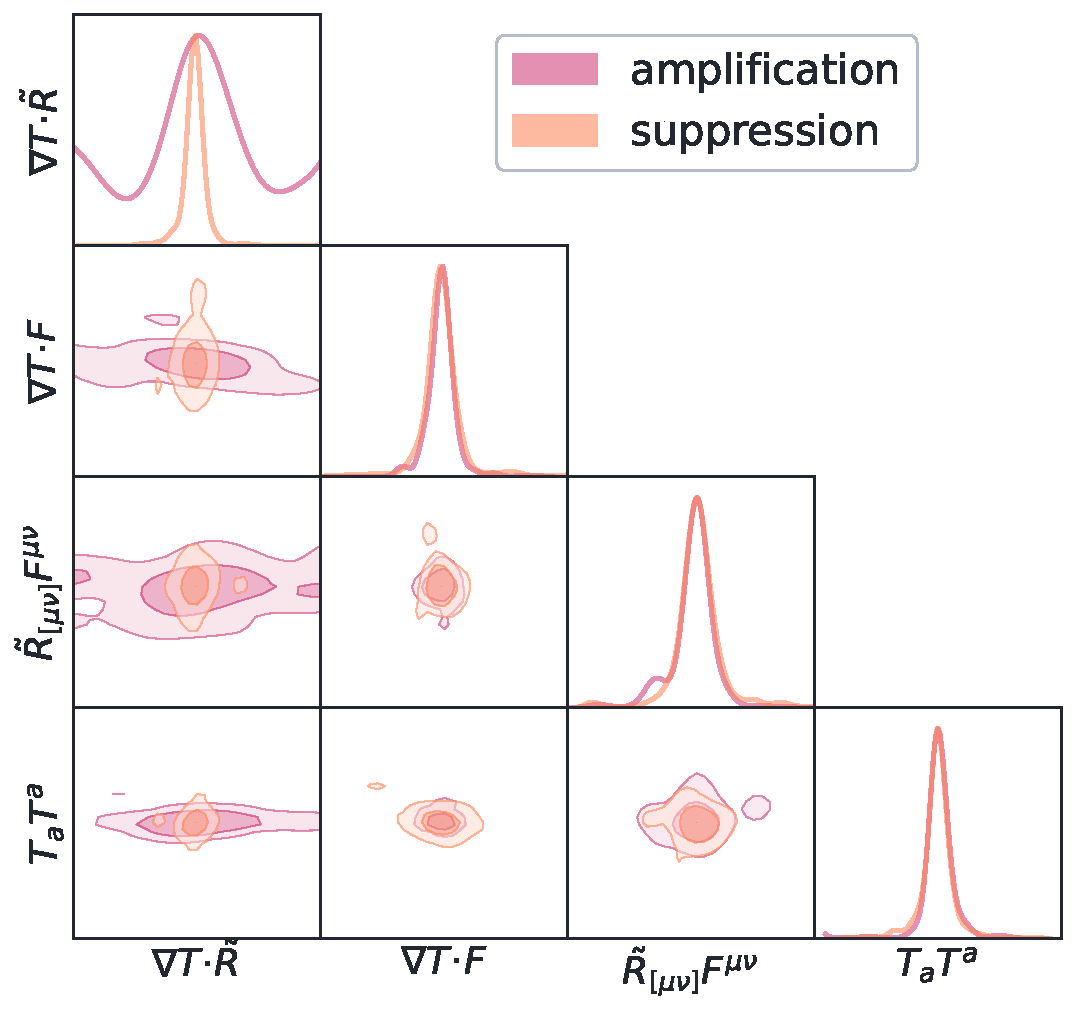
\includegraphics[width=\linewidth]{result_landscape.pdf}
    \end{column}
    % --- interpretation + dominant operator ---
    \begin{column}{0.38\linewidth}
      \raggedright
      The conversion responds to the full content of
      each theory, but a few operators are \emph{robustly dominant}. The most
      consistent amplifier is
      \vspace{0.8ex}

      % Dominant-operator equation inside a padded coloured box (a plain
      % beamercolorbox, so the display equation cannot escape below the fill).
      {\centering
        \begin{beamercolorbox}[wd=\linewidth,sep=1.6ex,center]{eqn box}
          % \resizebox scales the equation to the box width on a SINGLE line --
          % maximally large for emphasis, and guaranteed never to wrap (the column
          % is too narrow for a fixed \Huge/\huge, which broke after \supset).
          \resizebox{0.92\linewidth}{!}{%
            $\lag \;\supset\; \rcD{^{\alpha}}\MAGT{^{\beta\gamma\delta}}\,
              \MAGF{_{\alpha\beta\gamma\delta}}$}
        \end{beamercolorbox}\par}
      \vspace{0.8ex}
      Some directions in the coupling space \textbf{amplify} the conversion and
      others \textbf{suppress} it --- distinct regions, not a single effect. The
      amplification persists without
      propagating-torsion, so purely ghost-driven growth cannot explain it.
    \end{column}
  \end{columns}
\end{block}

  \end{column}
  \separatorcolumn
\end{columns}

% ---- Row 4: outlook + references -------------------------------------------
\begin{columns}[t]
  \separatorcolumn
  \begin{column}{\dimexpr\paperwidth-2\sepwidth\relax}
    % Outlook + references + QR (footer strip above the theme footline).
\begin{columns}[t]
  \begin{column}{0.62\linewidth}
    \begin{block}{Outlook}
      A magnetic field of \emph{finite extent} gives the wave a finite
      interaction time, bounding the growth and turning these amplifications
      into physical conversion magnitudes --- the operators ranked here are the
      inputs that calculation needs. A particle-spectrum analysis
      (\PSALTer{}) will then classify each amplifying direction.
    \end{block}
  \end{column}
  \begin{column}{0.24\linewidth}
    \begin{block}{References}
      \footnotesize
      Gertsenshtein, \emph{JETP}, 1962.\\
      Boccaletti \etal, \emph{Nuovo Cim.}, 1970.\\
      Barker \etal, \emph{PSALTer}, 2024,\\ arXiv:2406.09500.
    \end{block}
  \end{column}
  \begin{column}{0.10\linewidth}
    \centering
    \qrcode[height=4cm]{https://github.com/WilliamRoyce/torsion-gertsenshtein}\\[0.3ex]
    {\footnotesize Code \& data}
  \end{column}
\end{columns}

  \end{column}
  \separatorcolumn
\end{columns}

\end{frame}
\end{document}
